% !TeX program = xelatex
\documentclass[a4paper,10pt]{article}

% ============================================================================
% សន្លឹកកិច្ចការសិស្ស ស-ខ្មៅ (Student Guided-Inquiry Worksheet - Grade 8 ALG56)
% បរិបទ៖ ថ្នាក់រៀនគ្មានស្លាយ LCD – ៣.២ ពន្លាតគូបនៃទ្វេធា និងត្រីកោណប៉ាស្កាល់ (២ ទំព័រ A4)
% ============================================================================
\usepackage[a4paper, left=0.90cm, right=0.90cm, top=0.75cm, bottom=0.85cm, footskip=0.45cm]{geometry}
\usepackage{amsmath, amssymb}
\usepackage{unicode-math}
\usepackage{fontspec}
\usepackage{array, colortbl}
\usepackage[table]{xcolor}
\usepackage{enumitem}
\usepackage{pifont}
\usepackage{fancyhdr}
\usepackage{lastpage}
\usepackage{tikz}
\usepackage[most]{tcolorbox}
\usetikzlibrary{calc, arrows.meta, positioning, babel}

\makeatletter
\let\@expl@@@mark@update@singlecol@structures@@\relax
\makeatother

\providecommand{\NGSFindFonts}{%
  \IfFileExists{C:/Windows/Fonts/cambria.ttc}{%
    \def\NGSSysPath{C:/Windows/Fonts/}%
    \def\NGSUserPath{C:/Users/KIT/AppData/Local/Microsoft/Windows/Fonts/}%
  }{%
    \IfFileExists{./fonts/KhmerOSsiemreap.ttf}{\def\NGSSysPath{./fonts/}\def\NGSUserPath{./fonts/}}{%
    \IfFileExists{../fonts/KhmerOSsiemreap.ttf}{\def\NGSSysPath{../fonts/}\def\NGSUserPath{../fonts/}}{%
    \IfFileExists{../../fonts/KhmerOSsiemreap.ttf}{\def\NGSSysPath{../../fonts/}\def\NGSUserPath{../../fonts/}}{%
    \IfFileExists{../../../fonts/KhmerOSsiemreap.ttf}{\def\NGSSysPath{../../../fonts/}\def\NGSUserPath{../../../fonts/}}{%
    \IfFileExists{../../../../fonts/KhmerOSsiemreap.ttf}{\def\NGSSysPath{../../../../fonts/}\def\NGSUserPath{../../../../fonts/}}{%
    \IfFileExists{../../../../../fonts/KhmerOSsiemreap.ttf}{\def\NGSSysPath{../../../../../fonts/}\def\NGSUserPath{../../../../../fonts/}}{%
    \IfFileExists{../../../../../../fonts/KhmerOSsiemreap.ttf}{\def\NGSSysPath{../../../../../../fonts/}\def\NGSUserPath{../../../../../../fonts/}}{%
      \def\NGSSysPath{../../../../../../../fonts/}\def\NGSUserPath{../../../../../../../fonts/}%
    }}}}}}}%
  }%
}
\NGSFindFonts

\setmathfont[Path={\NGSSysPath}, FontIndex=1, Scale=1.02]{cambria.ttc}
\defaultfontfeatures{Ligatures=TeX}

\setmainfont[
  Path={\NGSUserPath},
  Extension=.ttf,
  Script=Khmer,
  BoldFont={KhmerOSsiemreap},
  BoldFeatures={FakeBold=1.8},
  ItalicFont={KhmerOSsiemreap},
  ItalicFeatures={FakeSlant=0.25},
  BoldItalicFont={KhmerOSsiemreap},
  BoldItalicFeatures={FakeBold=1.8, FakeSlant=0.25}
]{KhmerOSsiemreap}

\newfontfamily\muol[Path={\NGSUserPath}, Extension=.ttf, Script=Khmer]{KhmerOSmuollight}
\newfontfamily\TimesEn[Path={\NGSSysPath}, Extension=.ttf, BoldFont={timesbd}, ItalicFont={timesi}, BoldItalicFont={timesbi}]{times}

\XeTeXlinebreaklocale "km"
\XeTeXlinebreakskip = 0pt plus 1pt minus 0.1pt

\definecolor{panelgray}{gray}{0.94}
\definecolor{headgray}{gray}{0.86}

\pagestyle{fancy}
\fancyhf{}
\renewcommand{\headrulewidth}{0pt}
\fancyfoot[L]{\fontsize{8pt}{10pt}\selectfont អនុវិទ្យាល័យព្រះក្រសាំង \en{|} គណិតវិទ្យា ថ្នាក់ទី៨ \en{|} មេរៀនទី៥ (៣.២ ពន្លាតគូបនៃទ្វេធា និងត្រីកោណប៉ាស្កាល់)}
\fancyfoot[R]{\fontsize{8.2pt}{10pt}\selectfont ទំព័រ \en{\thepage\ / \pageref{LastPage}}}

\setlength{\parindent}{0pt}
\setlength{\parskip}{0pt}
\setlength{\tabcolsep}{4pt}

\newcommand{\en}[1]{{\TimesEn #1}}
\newcommand{\enbf}[1]{{\TimesEn\textbf{#1}}}
\newcommand{\unit}[1]{\,\text{\en{#1}}}
\newcommand{\cnum}[1]{{\fontsize{10pt}{12pt}\selectfont\ding{\numexpr171+#1\relax}}}
\newcommand{\chk}{\tikz[baseline=-0.15ex]\draw[black, line width=0.8pt] (0,0) rectangle (0.25cm,0.25cm);}
\newcommand{\dotline}[1]{\makebox[#1]{\dotfill}}

\newcolumntype{L}[1]{>{\raggedright\arraybackslash}p{#1}}
\newcolumntype{C}[1]{>{\centering\arraybackslash}p{#1}}

\newcommand{\secbar}[2]{%
  \vspace{5pt}
  \noindent\colorbox{headgray}{\parbox{\dimexpr\linewidth-2\fboxsep\relax}{%
    \vspace{1.8pt}{\muol\fontsize{9.5pt}{13.5pt}\selectfont #1}\hfill{\fontsize{8.5pt}{12pt}\selectfont\textbf{#2}}\vspace{1.8pt}%
  }}\par\vspace{5pt}
}

\begin{document}
\fontsize{9.5pt}{14.2pt}\selectfont

% ============================================================================
% ទំព័រទី១៖ ក្បាលសន្លឹកកិច្ចការ + E1 + E2 + E3
% ============================================================================
\begin{tcolorbox}[enhanced, sharp corners, colback=white, colframe=black, boxrule=1.0pt, top=4pt, bottom=4pt, left=6pt, right=6pt]
  \begin{center}
    {\muol\fontsize{10.5pt}{15pt}\selectfont សន្លឹកកិច្ចការសិស្ស — មេរៀនទី៥៖ កន្សោមពីជគណិត \enbf{(}៣.២ គូបនៃទ្វេធា និងត្រីកោណប៉ាស្កាល់\enbf{)}}\\[2pt]
    {\footnotesize សៀវភៅសិក្សាគោលថ្នាក់ទី៨ ទំព័រ ៦៦--៦៨ \en{|} លំនាំមេគុណត្រីកោណប៉ាស្កាល់ និងការស៊ីសងតួកណ្ដាល (គ្មានស្លាយ \en{LCD})}
  \end{center}
  \vspace{2pt}
  \hrule height 0.5pt
  \vspace{4pt}
  ឈ្មោះសិស្ស៖ \dotline{5.3cm} ថ្នាក់៖ \dotline{2.0cm} ដៃគូទី៖ \dotline{2.0cm} កាលបរិច្ឆេទ៖ \dotline{3.3cm}
\end{tcolorbox}

% -------------------- ផ្នែកទី១៖ E1 ENGAGE --------------------
\secbar{ផ្នែកទី១ ៖ បេសកកម្មភ្ជាប់បញ្ហា \enbf{(E1 — Engage)} — អាថ៌កំបាំងមេគុណទ្វេធា និងអន្ទាក់គូប}{\en{3} នាទី (ទស្សន៍ទាយមុនរៀន)}

\begin{tcolorbox}[enhanced, sharp corners, colback=panelgray, colframe=black, boxrule=0.8pt, top=3.5pt, bottom=3.5pt, left=6pt, right=6pt]
  \begin{minipage}[c]{12.8cm}
    ១) ផ្ទៀងផ្ទាត់លេខ៖ $(2 + 1)^3 = 3^3 = \dotline{1.2cm}$ ខណៈ $2^3 + 1^3 = 8 + 1 = \dotline{1.2cm}$ $\implies$ $(a+b)^3 \ne a^3 + b^3$!\\[2pt]
    ២) \textbf{ទស្សន៍ទាយមេគុណ៖} បើ $(x+1)^1 = 1x+1$ និង $(x+1)^2 = 1x^2+2x+1$ តើមេគុណនៃ $(x+1)^3$ ស្មើប៉ុន្មាន?\\[1.5pt]
    \hspace*{0.3cm}\chk\ $1,\; 1$ \qquad\qquad
    \chk\ $1,\; 2,\; 2,\; 1$ \qquad\qquad
    \chk\ $1,\; 3,\; 3,\; 1$
  \end{minipage}\hfill
  \begin{minipage}[c]{5.4cm}
    \centering
    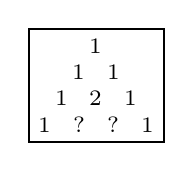
\begin{tikzpicture}
      \node[draw=black, line width=0.8pt, fill=white, inner sep=3.5pt, font=\footnotesize, align=center] {
        $1$\\
        $1 \quad 1$\\
        $1 \quad 2 \quad 1$\\
        $1 \quad ? \quad ? \quad 1$
      };
    \end{tikzpicture}
  \end{minipage}
\end{tcolorbox}

% -------------------- ផ្នែកទី២៖ E2 EXPLORE --------------------
\secbar{ផ្នែកទី២ ៖ រុករកសមភាពគូបទាំង ៤ និងត្រីកោណប៉ាស្កាល់ \enbf{(E2 — Explore)}}{\en{11} នាទី (ពិភាក្សាដៃគូ)}

\textbf{ក. សកម្មភាពទី១ (រុករកគូបនៃផលបូក ទំ.៦៦ និងគូបនៃផលដក ទំ.៦៦--៦៧)៖}
\begin{enumerate}[label=\arabic*., leftmargin=0.55cm, itemsep=4.5pt, topsep=2pt]
  \item \textbf{ពន្លាត $(a+b)^3$៖} ដោយ $(a+b)^3 = (a+b)^2(a+b) = (a^2 + 2ab + b^2)(a + b)$ ចូរបង្រួមតួដូចគ្នា៖\\
  $= a^3 + 2a^2b + ab^2 + a^2b + 2ab^2 + b^3 = a^3 + \dotline{1.8cm} + \dotline{1.8cm} + b^3$ \quad \textbf{រូបមន្ត \en{(4)}} ។
  \item \textbf{ពន្លាត $(a-b)^3$៖} ដោយ $(a-b)^3 = (a-b)(a^2 - 2ab + b^2)$ ចូរបង្រួមតួដូចគ្នា៖\\
  $= a^3 - 2a^2b + ab^2 - a^2b + 2ab^2 - b^3 = a^3 - \dotline{1.8cm} + \dotline{1.8cm} - b^3$ \quad \textbf{រូបមន្ត \en{(5)}} ។
  \item \textbf{សង្កេតសញ្ញា និងផ្ទៀងផ្ទាត់លេខ៖} ក្នុង $(a-b)^3$ សញ្ញាឆ្លាស់គ្នាតាមលំដាប់ $+\;,\; \dotline{0.8cm}\;,\; \dotline{0.8cm}\;,\; \dotline{0.8cm}$ ។ ផ្ទៀងផ្ទាត់ចំពោះ $a=2, b=1$៖ $(2+1)^3 = 2^3 + 3(2^2)(1) + 3(2)(1^2) + 1^3 = 8 + \dotline{1.0cm} + \dotline{1.0cm} + 1 = \dotline{1.1cm}$ ។
\end{enumerate}

\vspace{5pt}
\textbf{ខ. សកម្មភាពទី២ (រុករកផលគុណបង្កើតផលដកពីរគូប $a^3-b^3$ និងផលបូកពីរគូប $a^3+b^3$ ទំ.៦៧)៖}
\begin{enumerate}[label=\arabic*., leftmargin=0.55cm, itemsep=4.5pt, topsep=2pt]
  \item \textbf{គូសឈូតតួផ្ទុយគ្នាក្នុង $(a-b)(a^2+ab+b^2)$៖}\\
  $= a^3 + a^2b + ab^2 - a^2b - ab^2 - b^3 = \dotline{3.0cm}$ \quad \textbf{រូបមន្ត \en{(6)}} (ផលដកនៃពីរគូប) ។
  \item \textbf{គូសឈូតតួផ្ទុយគ្នាក្នុង $(a+b)(a^2-ab+b^2)$៖}\\
  $= a^3 - a^2b + ab^2 + a^2b - ab^2 + b^3 = \dotline{3.0cm}$ \quad \textbf{រូបមន្ត \en{(7)}} (ផលបូកនៃពីរគូប) ។
  \item \textbf{ប្រៀបធៀបសញ្ញា៖} បើទ្វេធាមានសញ្ញាដក $(a-b)$ នោះត្រីធាត្រូវមានសញ្ញា $\dotline{1.2cm}$ ទាំងអស់ \;,\; តែបើទ្វេធាមានសញ្ញាបូក $(a+b)$ នោះតួកណ្ដាលនៃត្រីធាត្រូវមានសញ្ញា $\dotline{1.2cm}$ (ទើបស៊ីសងតួកណ្ដាលអស់សូន្យ!) ។
\end{enumerate}

\vspace{5pt}
% -------------------- ផ្នែកទី៣៖ E3 EXPLAIN --------------------
\secbar{ផ្នែកទី៣ ៖ រូបមន្តសង្ខេប \enbf{(4)--(7)} និងត្រីកោណប៉ាស្កាល់ \enbf{(E3 — Explain)}}{\en{6} នាទី (កត់ត្រាខ្លឹមសារគោល)}

\begin{tcolorbox}[enhanced, sharp corners, colback=white, colframe=black, boxrule=0.85pt, top=5.5pt, bottom=5.5pt, left=6pt, right=6pt]
  \begin{minipage}[c]{11.8cm}
    \cnum{1} \textbf{គូបនៃផលបូក \en{(4)}៖} $(a + b)^3 = \dotline{5.2cm}$\\[4.5pt]
    \cnum{2} \textbf{គូបនៃផលដក \en{(5)}៖} $(a - b)^3 = \dotline{5.2cm}$\\[4.5pt]
    \cnum{3} \textbf{ផលដកពីរគូប \en{(6)}៖} $(a - b)(a^2 + ab + b^2) = \dotline{3.2cm}$\\[4.5pt]
    \cnum{4} \textbf{ផលបូកពីរគូប \en{(7)}៖} $(a + b)(a^2 - ab + b^2) = \dotline{3.2cm}$\\[4.5pt]
    \cnum{5} \textbf{ត្រីកោណប៉ាស្កាល់ (ទំ.៦៨)៖} បំពេញមេគុណដែលបាត់នៅជួរទី៤ និងទី៥ ខាងស្ដាំ!
  \end{minipage}\hfill
  \begin{minipage}[c]{6.0cm}
    \centering
    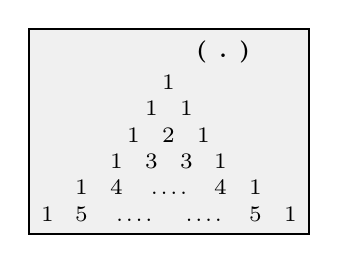
\begin{tikzpicture}
      \node[draw=black, line width=0.8pt, fill=panelgray, inner sep=4.5pt, font=\footnotesize, align=center] {
        \textbf{ត្រីកោណប៉ាស្កាល់ (ទំ.៦៨)}\\[2pt]
        $1$\\
        $1 \quad 1$\\
        $1 \quad 2 \quad 1$\\
        $1 \quad 3 \quad 3 \quad 1$\\
        $1 \quad 4 \quad \dotline{0.6cm} \quad 4 \quad 1$\\
        $1 \quad 5 \quad \dotline{0.6cm} \quad \dotline{0.6cm} \quad 5 \quad 1$
      };
    \end{tikzpicture}
  \end{minipage}\\[5pt]
  \centering
  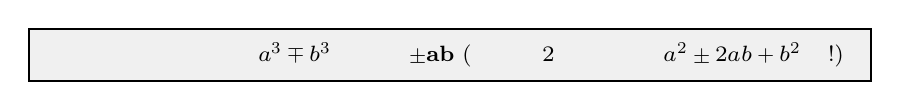
\begin{tikzpicture}
    \node[draw=black, line width=0.8pt, fill=panelgray, inner xsep=10pt, inner ysep=5pt, font=\footnotesize] {ចំណាំកុំឱ្យច្រឡំ៖ ក្នុងត្រីធានៃ $a^3 \mp b^3$ តួកណ្ដាលគឺ $\mathbf{\pm ab}$ (\textbf{គ្មានមេគុណ $2$} ដូចការេនៃទ្វេធា $a^2 \pm 2ab + b^2$ ឡើយ!)};
  \end{tikzpicture}
\end{tcolorbox}

\newpage
% ============================================================================
% ទំព័រទី២៖ E4 (លំហាត់គំរូ ទំ.៦៦-៦៨) + E5 (ប្រតិបត្តិ + Exit Check) + កិច្ចការផ្ទះ
% ============================================================================

% -------------------- ផ្នែកទី៤៖ E4 ELABORATE --------------------
\secbar{ផ្នែកទី៤ ៖ អនុវត្តលំហាត់គំរូ និងត្រីកោណប៉ាស្កាល់ \enbf{(E4 — Elaborate)}}{\en{10} នាទី (បំពេញតាមគំរូ)}

\textbf{១. លំហាត់គំរូតាមសៀវភៅគោល (ទំ.៦៦--៦៧)៖}
\begin{itemize}[leftmargin=0.5cm, itemsep=4.5pt, topsep=2pt]
  \item \textbf{គំរូ \en{(4)} និង \en{(5)}៖} $(x + 1)^3 = \dotline{4.5cm}$ \;;\; $(x - 1)^3 = \dotline{4.5cm}$ ។
  \item \textbf{គំរូ \en{(6)} និង \en{(7)}៖} $(x - 1)(x^2 + x + 1) = \dotline{2.6cm}$ \;;\; $(x + 1)(x^2 - x + 1) = \dotline{2.6cm}$ ។
  \item \textbf{អនុវត្តមានប្រភាគ (ទំ.៦៦)៖} $\left(\dfrac{1}{5}a + b\right)^3 = \left(\dfrac{1}{5}a\right)^3 + 3\left(\dfrac{1}{5}a\right)^2 b + 3\left(\dfrac{1}{5}a\right)b^2 + b^3 = \dotline{4.6cm}$ ។
  \item \textbf{អនុវត្តមានរ៉ាឌីកាល់ (ទំ.៦៧)៖} $(\sqrt{2}a - 3b)(2a^2 + 3\sqrt{2}ab + 9b^2) = (\sqrt{2}a)^3 - (3b)^3 = \dotline{3.8cm}$ ។
  \item \textbf{គិតលេខមាត់តាមគូបនៃទ្វេធា៖} $11^3 = (10+1)^3 = 1000 + \dotline{1.2cm} + \dotline{1.1cm} + 1 = \dotline{1.6cm}$ ។
\end{itemize}

\vspace{4.5pt}
\textbf{២. ការពន្លាត $(x+1)^4$ និង $(x+1)^5$ ដោយប្រើត្រីកោណប៉ាស្កាល់ (សៀវភៅគោល ទំ.៦៨)៖}
\begin{itemize}[leftmargin=0.5cm, itemsep=4.5pt, topsep=2pt]
  \item ប្រើជួរទី៤ ($1, 4, 6, 4, 1$)៖ $(x + 1)^4 = x^4 + \dotline{1.3cm} + \dotline{1.3cm} + \dotline{1.3cm} + 1$ ។
  \item ប្រើជួរទី៥ ($1, 5, 10, 10, 5, 1$)៖ $(x + 1)^5 = x^5 + \dotline{1.3cm} + \dotline{1.5cm} + \dotline{1.5cm} + \dotline{1.3cm} + 1$ ។
  \item \textbf{ឆ្លុះបញ្ចាំង (\en{Looking Back})៖} ក្នុងពន្លាត $(a + b)^n$ ផលបូកនិទស្សន្តនៃ $a$ និង $b$ ក្នុងតួនីមួយៗស្មើ $\dotline{1.2cm}$ ជានិច្ច ហើយចំនួនតួសរុបស្មើ $n + \dotline{0.9cm}$ តួ!
\end{itemize}

% -------------------- ផ្នែកទី៥៖ E5 EVALUATE --------------------
\secbar{ផ្នែកទី៥ ៖ ហ្វឹកហាត់ «ប្រតិបត្តិ» និងតេស្តរហ័ស \enbf{(E5 — Evaluate)}}{\en{10} នាទី (ធ្វើដោយខ្លួនឯង រួចប្ដូរផ្ទៀង)}

\textbf{១. ប្រតិបត្តិពន្លាតគូបនៃទ្វេធា (ទំ.៦៦--៦៧) និងផលគុណបង្កើតគូប (ទំ.៦៧)៖}

\vspace{2pt}
{\renewcommand{\arraystretch}{1.48}
\begin{tabular}{|L{9.1cm}|L{9.1cm}|}
\hline
\cellcolor{headgray}\textbf{ប្រតិបត្តិគូបនៃទ្វេធា \en{(4)--(5)} (ទំ.៦៦--៦៧)} & \cellcolor{headgray}\textbf{ប្រតិបត្តិផលគុណបង្កើតគូប \en{(6)--(7)} (ទំ.៦៧)} \\
\hline
ក. $(x + 2y)^3 = \dotline{5.5cm}$ & ក. $(a - 1)(a^2 + a + 1) = \dotline{3.8cm}$ \\
\hline
ខ. $(x + 3y)^3 = \dotline{5.5cm}$ & ខ. $(x - 3)(x^2 + 3x + 9) = \dotline{3.6cm}$ \\
\hline
គ. $(3x + 4y)^3 = \dotline{5.3cm}$ & គ. $(2x - 1)(4x^2 + 2x + 1) = \dotline{3.1cm}$ \\
\hline
ឃ. $(3x - 2y)^3 = \dotline{5.3cm}$ & ឃ. $(a + 1)(a^2 - a + 1) = \dotline{3.8cm}$ \\
\hline
ង. $(2x - y)^3 = \dotline{5.5cm}$ & ង. $(x + 3)(x^2 - 3x + 9) = \dotline{3.5cm}$ \\
\hline
\cellcolor{panelgray}គិតមាត់៖ $11^3 = (10+1)^3 = \dotline{4.0cm}$ & ច. $(2x + 1)(4x^2 - 2x + 1) = \dotline{3.1cm}$ \\
\hline
\end{tabular}}

\vspace{4pt}
\begin{tcolorbox}[enhanced, sharp corners, colback=panelgray, colframe=black, boxrule=0.85pt, top=3pt, bottom=3pt, left=6pt, right=6pt]
  \textbf{២. បិទបេសកកម្ម \en{E1} និងតេស្តរហ័ស (\en{Exit Check — 60} វិនាទី)៖}\\[2pt]
  $\bullet$ \textbf{ចម្លើយបេសកកម្ម \en{E1}៖} មេគុណនៃ $(x+1)^3$ គឺ $\dotline{2.5cm}$ ហើយ $(2+1)^3 = 8 + 12 + 6 + 1 = \dotline{1.2cm}$ ។\\[2pt]
  $\bullet$ \textbf{សំណួរតេស្តរហ័ស៖} តើផលគុណ $(2x + 3)(4x^2 - 6x + 9)$ ស្មើនឹងកន្សោមមួយណា? (គូសរង្វង់ជម្រើសត្រឹមត្រូវ)\\[1.5pt]
  \hspace*{0.3cm}\enbf{A.}\; $8x^3 - 27$ \qquad\quad
  \enbf{B.}\; $2x^3 + 27$ \qquad\quad
  \enbf{C.}\; $8x^3 + 27$ \qquad\quad
  \enbf{D.}\; $8x^3 + 12x^2 + 27$
\end{tcolorbox}

% -------------------- ផ្នែកទី៦៖ កិច្ចការផ្ទះ --------------------
\secbar{ផ្នែកទី៦ ៖ ប័ណ្ណកិច្ចការផ្ទះ \enbf{(Homework)} និងការអានជាមុន}{សៀវភៅសិក្សាគោល ទំ.៦៦--៦៧ និងទំ.៧៣}

\begin{tcolorbox}[enhanced, sharp corners, colback=white, colframe=black, boxrule=0.8pt, borderline={0.6pt}{2pt}{dashed}, top=3pt, bottom=3pt, left=6pt, right=6pt]
  \textbf{១. ប្រតិបត្តិ ឃ (ទំ.៦៦--៦៧)៖} ពន្លាត $\left(\dfrac{1}{5}a + b\right)^3$, $\left(\dfrac{1}{5}t - k\right)^3$ និង $(\sqrt{2}a + 3b)(2a^2 - 3\sqrt{2}ab + 9b^2)$ ។\\[1.5pt]
  \textbf{២. លំហាត់ទី១០ ង (ទំ.៧៣)៖} ពន្លាត និងបង្រួមតាមលំដាប់ដឺក្រេ៖ $(x - 1)^3 - (x + 2)^3$ ។\\[1.5pt]
  \textbf{៣. ត្រីកោណប៉ាស្កាល់៖} រកជួរទី៦ នៃត្រីកោណប៉ាស្កាល់ រួចសរសេរពន្លាតនៃ $(x + 1)^6$ ។\\[1.5pt]
  $\bullet$ \textbf{អានជាមុន៖} ចំណុច \textbf{៤.១ និង ៤.២ ការដាក់ជាផលគុណកត្តាដោយកត្តារួម និងតាមសមភាពសំខាន់ៗ} (សៀវភៅគោល ទំព័រ ៦៨--៧០) ។
\end{tcolorbox}

\end{document}
